\subsection{Validazione}
\subsubsection{Scopo}
Questo processo assicura che il prodotto rispetti i requisiti e soddisfi le aspettative del proponente.

\subsubsection{Descrizione}
Per svolgere quanto sopra descritto si  usa come input l'output del processo di verifica,
restituendolo con la garanzia che soddisfi i requisiti.\\
Il principale attore è il \textit{Responsabile di Progetto}, il quale ha l'onere di decidere
se accettare e quindi approvare il prodotto oppure rigettarlo, indicando quali verifiche sono mancanti.

\subsubsection{Aspettative}
Per avviare il processo di validazione devono essere presenti questi elementi:
\begin{itemize}
    \item Identificazione degli elementi da validare (documenti e/o codice sorgente);
    \item Adottare una strategia di validazione che permetta di riutilizzare le procedure usate
          per la validazione;
    \item Valutazione dei risultati rispetto alle attese.
\end{itemize}

\subsubsection{Validazione dei documenti}
\begin{figure}[h!]
    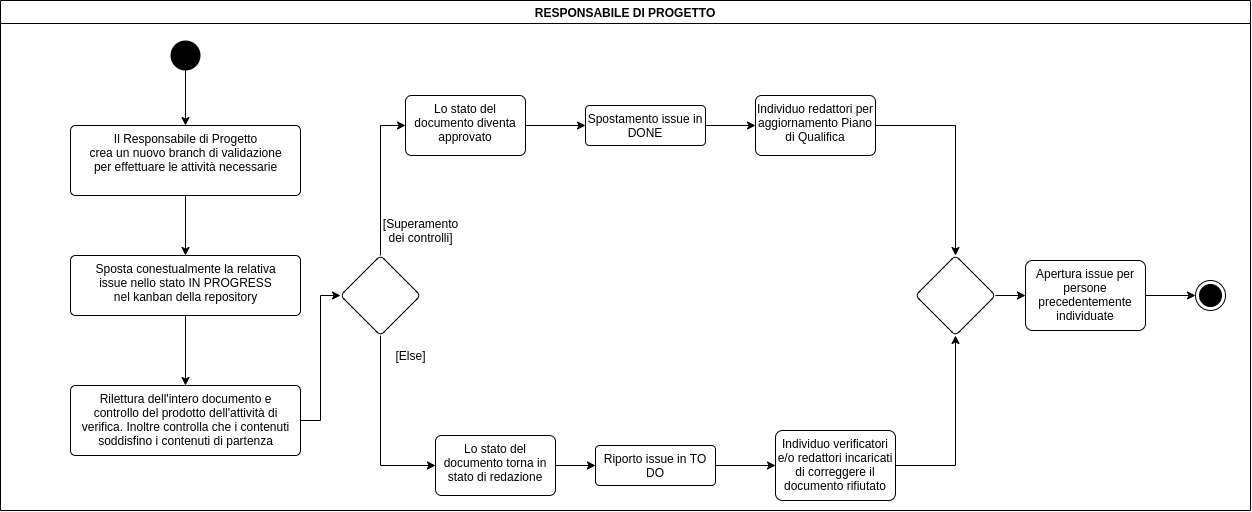
\includegraphics[width=\linewidth]{res/images/processo_validazione.png}
    \caption{Processo di validazione documenti}
\end{figure}

% \subsubsection{Attività per la validazione}

% \subsubsection{Test di validazione}

% \subsubsection{Responsabilità dei test}

% \paragraph{Codice identificativo dei test}
% Ogni test è descritto mediante:
% \begin{itemize}
%     \item codice identificativo:
%     \item descrizione;
%     \item stato, che può essere:
%     \begin{itemize}
%         \item implementato;
%         \item non implementato;
%         \item superato;
%         \item non superato.
%     \end{itemize}
% \end{itemize}
% Il codice identificativo si presenta nella seguente forma:
% \begin{center}
%     \textbf{T[Tipo][ID]}
% \end{center}
% dove:
% \begin{itemize}
%     \item \textbf{Tipo}: indica la tipologia del test e può assumere i valori:
%     \begin{itemize}
%         \item \textbf{U}: test di unità;
%         \item \textbf{I}: test di integrazione;
%         \item \textbf{S}: test di sistema;
%         \item \textbf{R}: test di regressione;
%         \item \textbf{V}: test di validazione.
%     \end{itemize}
%     \item \textbf{ID}: i valori che questo può assumere sono:
%     \begin{itemize}
%         \item \textbf{IDNumerico}: se si tratta di un test di unità, di integrazione o di regressione. Viene espresso con un numero progressivo;
%         \item \textbf{IDRequisito}: per i test di validazione e di sistema. È composto da:
%         \begin{center}
%             \textbf{[Tipo][Importanza][Codice]} 
%         \end{center}
%         secondo quanto descritto in \ref{_processoAnalisiDeiRequisiti} e indica il codice del requisito.
%     \end{itemize}
% \end{itemize}
